\documentclass[a4paper, 10pt]{article}

\usepackage[margin = 1in]{geometry} % for spacing around
\usepackage{tabularx}
\usepackage{graphicx} % for including images in your pdfs
\usepackage{xcolor} % for including colors in your pdf
\usepackage{soul} % for text decoration
\usepackage[utf8]{inputenc} % for encoded text
\usepackage[T1]{fontenc}
\usepackage{setspace} % for setting different line spacings between paragrafs.
\usepackage{enumerate} % for letting us get more detailed enumerate lists
\usepackage{multirow} % to let us combine more rows together
\usepackage{colortbl} % for decorating tables
\usepackage{amsmath} % used for representing more complicated math displays
\usepackage{supertabular}
\usepackage{longtable} % both of these packages are used to making really big tables
\usepackage{wrapfig} % allows us to wrap text around figures
\usepackage{fancyhdr} % for making fancy headers
%\usepackage{bibtex} % for making better bibliographies
\usepackage[pdftex]{hyperref} % for letting us make links
\usepackage{lscape} % Allows us to flip from portrait to landspace
\usepackage{tikz} % for high detailed drawing
\usepackage{multicol} % To put things side by side
\usepackage{rotating} % For rotating objects
% \usepackage{draftwatermark} % For adding watermarks
\usepackage{MnSymbol} % for using multiple symbols
\usepackage{mathtools} % Used for more math symbols
\usepackage{xfrac} % For more complciated fractions and to add derivitives
\usepackage{hyperref} % for hyper links
\usepackage{enumitem} % for better enum lists
\usepackage{tcolorbox} % for adding colored text boxes
\usepackage{bm} % Adding bold text to math inputs
\usepackage{pgfplots} % Used for plotting functions
\usepackage{pgfplotstable} % Used for plotting tables
\usepackage{booktabs} % for nicer tables
\usepackage{longtable} % for long tables that can span multiple pages
\usepackage[toc,page]{appendix} % for adding appendices
\usepackage{array}
\usepackage{colortbl}
\usepackage{caption}
\usepackage{subcaption}
\usepackage{minted}
\usepackage{listings}

\definecolor{lightgray}{gray}{0.95}
\renewcommand{\arraystretch}{1.3}

% Setting up the default image path
\graphicspath{{./Images/}}

% Implementing authro details
\title{}
\author{}
\date{}

% Setting up the fancy page style
\fancypagestyle{customStyle}{
	\lhead{} \chead{} \rhead{}
	\lfoot{} \cfoot{\thepage} \rfoot{}
	\renewcommand{\headrulewidth}{0pt}
	\renewcommand{\footrulewidth}{1pt}
}
\pagestyle{customStyle}

% Setting up hyperref options
\hypersetup {
	colorlinks = false,
	citecolor = black,
	filecolor = blue,
	linkcolor = blue,
	urlcolor = blue,
	pdftex
}

% Custom commands

% Custom column colors
\definecolor{lightblue}{RGB}{220,230,255}
\definecolor{lightgreen}{RGB}{220,255,220}
\definecolor{lightyellow}{RGB}{255,250,210}
\definecolor{lightpink}{RGB}{255,230,230}

\definecolor{codegray}{gray}{0.95}
\definecolor{darkblue}{rgb}{0.0,0.0,0.5}
\definecolor{darkgreen}{rgb}{0.0,0.5,0.0}
\definecolor{darkred}{rgb}{0.5,0.0,0.0}

% Define a style for Python code
\lstdefinestyle{pythonstyle}{
  backgroundcolor=\color{codegray},   
  commentstyle=\color{darkgreen}\itshape,
  keywordstyle=\color{darkblue}\bfseries,
  stringstyle=\color{darkred},
  basicstyle=\ttfamily\footnotesize,
  breaklines=true,            % ENABLE LINE WRAPPING
  numbers=left,
  numbersep=5pt,
  showstringspaces=false,
  language=Python,
  frame=single
}

\begin{document}
	\begin{titlepage}
    \begin{center}
        
\includegraphics[width=0.6\textwidth]{IUS_Logo.png} \\[1.5cm]

        {\Huge \textbf{A Statistical Analysis of Public Tram Transportation in Sarajevo}} \\[1.2cm]

        {\LARGE \textbf{Statistical Modeling}} \\[0.5cm]
        {\Large MATH 306} \\[2cm]

        {\Large \textbf{International University of Sarajevo}} \\[0.3cm]
        {\large \today}
    \end{center}

		\vfill

		\begin{minipage}[t]{0.4\textwidth}
			\begin{flushleft} \large
				\textbf{Students:} \\
				\begin{itemize}
					\item Sanjin Ruzic 
					\item Emre Arapcic-Uevak 
				\end{itemize}
			\end{flushleft}
		\end{minipage}
		\hfill
		\begin{minipage}[t]{0.4\textwidth}
			\begin{flushright} \large
				\textbf{Professor:} \\
				\vspace{3mm}
				Dr. Ozge Buyukdagli
			\end{flushright}
		\end{minipage}
	\end{titlepage}
	\pagebreak
	
	\tableofcontents
	\pagebreak
	
	\section{Introduction and Motivation}
		Our project focuses on performing a statistical analysis to evaluate the accuracy of the public transportation company GRAS's claim that the 
		\emph{average tram wait time} is \textbf{4 minutes}, including during rush hours. \\

		\noindent Based on personal experience and public perception, this figure appeared questionable, especially during peak traffic times, 
		which often feel significantly longer. Therefore, we set out to verify whether this 4-minute average holds true under different conditions. \\

		\noindent In addition to wait times, we were also interested in analyzing the proportion of old vs. new trams operating during rush hours, 
		non-rush hours, and overall. \\
		
		\noindent This distinction is important because older trams are generally not accessible 
		to people in wheelchairs, with the exception of a single retrofitted model known as the “JUMBO TRAM”, 
		which is \emph{rarely} seen in service. By examining the deployment of accessible (\emph{new}) trams across different time periods, we aim to assess how inclusive the current tram system is for passengers with mobility impairments.

	\section{Defined Hypotheses}
		\subsection{Proportion of Old vs. New Trams}
			\label{sec:proportion_hypothesis}
			\begin{itemize}
					\item \textbf{Null Hypothesis ($H_0$):} The proportion of old and new trams is the same during rush and non-rush hours. ($p_{\text{old, rush}} = p_{\text{old, non-rush}}$)
					\item \textbf{Alternative Hypothesis ($H_a$):} The proportion of old trams is higher. ($p_{\text{old, rush}} > p_{\text{old, non-rush}}$)
			\end{itemize}

		\subsection{Average Tram Wait Time (Overall)}
			\label{sec:wait_time_hypothesis}
			\begin{itemize}
					\item \textbf{Null Hypothesis ($H_0$):} The average tram wait time, in general, is 4 minutes. ($\mu_0 = 4$)
					\item \textbf{Alternative Hypothesis ($H_a$):} The average tram wait time is not 4 minutes. ($\mu_a \neq 4$)
			\end{itemize}

		\subsection{Average Wait Time: Rush vs. Non-Rush Hours}
			\label{sec:wait_time_rush_non_rush_hypothesis}
			\begin{itemize}
					\item \textbf{Null Hypothesis ($H_0$):} The average wait time is the same during rush and non-rush hours. ($\mu_{\text{rush}} = \mu_{\text{non-rush}}$)
					\item \textbf{Alternative Hypothesis ($H_a$):} The average wait time is not the same during rush and non-rush hours. ($\mu_{\text{rush}} \neq \mu_{\text{non-rush}}$)
			\end{itemize}

		\subsection{Tram type distribution by time of day}
			\label{sec:tram_type_distribution_hypothesis}
			\begin{itemize}
					\item \textbf{Null Hypothesis ($H_0$):} The time of day does not significantly affect the distribution of tram types.
					\item \textbf{Alternative Hypothesis ($H_a$):} The time of day significantly affects the distribution of tram types.
			\end{itemize}

	\section{Data Description and Assumptions}

		\begin{spacing}{1.2}
			To collect the data for our analysis, we conducted \textbf{direct observation} at a tram station. 
			\noindent We waited for the \textbf{first tram to arrive} and used its departure as the \textbf{starting point} for our data collection. 
			After the reference tram left, we started a timer and recorded the \textbf{arrival time of the next tram}. 
			This process was repeated to collect multiple data points on tram arrival intervals. \\

			\noindent It is important to note that the \textbf{reference trams} (i.e., the first trams used to start each measurement cycle) were 
			\textbf{not included} in the dataset for average wait time calculations, but they were 
			\textbf{included in the population proportion analysis} (e.g., counting the number of old vs. new trams). \\

			\noindent We did not conduct surveys or use digital scheduling data; instead, all data was manually recorded based on real-time observations.
		\end{spacing}

			\subsection*{Assumptions and Limitations}
				We assume that:
				\begin{itemize}
						\item Tram arrivals are \textbf{independent} of one another.
						\item Our observation window is \textbf{representative} of general traffic conditions.
						\item Our sampling method is \textbf{non-random but unbiased} in timing—we observed whatever trams happened to arrive, without prior selection.
				\end{itemize}

				\noindent However, there are a few potential \textbf{biases and limitations}:
				\begin{itemize}
						\item \textbf{Rush hour vs. non-rush hour} boundaries were estimated based on perception, not official schedules.
						\item \textbf{External conditions} (e.g., traffic, weather, or delays) may have influenced tram arrivals during data collection.
						\item Data was collected \textbf{manually}, introducing possible human error in timing or tram classification.
				\end{itemize}

				\noindent Despite these limitations, the methodology provides a solid foundation for testing the hypotheses regarding wait times and tram accessibility. \\

				\noindent The raw data table containing all measurements is provided in \textbf{Appendix~\ref{sec:rawdata}}.

	\section{Descriptive Statistics and Visualizations}
		\subsection{Wait Time Distribution}
				To get a better understanding of the tram wait times,
				we plotted the distribution of wait times using a histogram. As can be seen in figure~\ref{fig:wait_time_distribution},
				the wait times are right-skewed, with most values clustered around 2-4 minutes.

				\begin{figure}[h!]
					\centering
					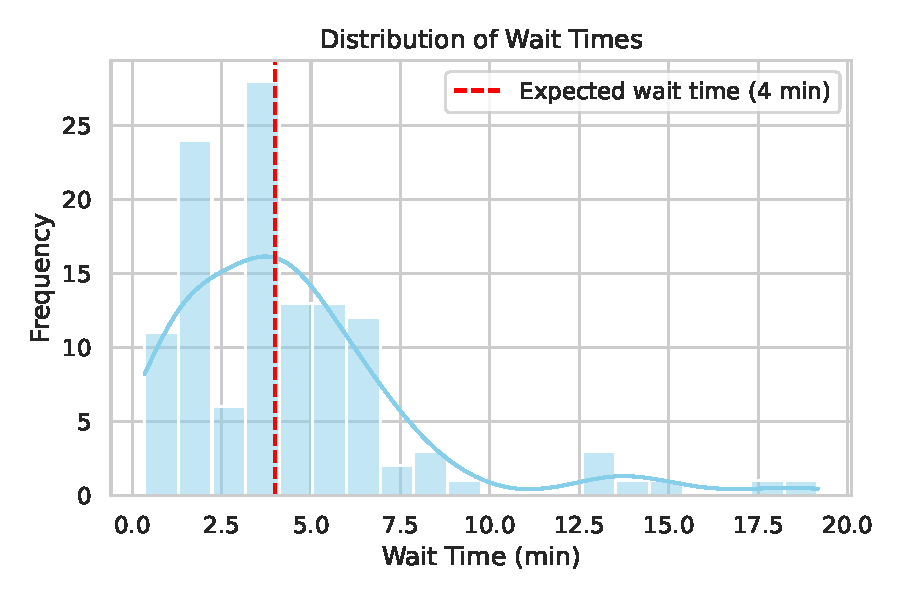
\includegraphics[width=0.8\textwidth]{Plot_DistributionOfWaitTimes.pdf}
					\caption{Distribution of Tram Wait Times}
					\label{fig:wait_time_distribution}
				\end{figure}

				\noindent We also marked the expected wait time of 4 minutes on the histogram to see if it is a reasonable estimate.
				And shockingly it is, even with all of the extreme values that we have because of the rush hour trams. \\
			
				\newpage

		\subsection{Wait Time Boxplot}
				To further analyze the tram wait times, we created two boxplot to visualize the distribution of wait times with respect
				to the type of the tram during rush hours and non-rush hours (Figure~\ref{fig:wait_time_by_tram_type}), 
				and with respect to the time of day (Figure~\ref{fig:wait_time_by_time_of_day}). \\

				\noindent The blue represents \textcolor{blue}{non rush hour} wait times, while the red 
				represents \textcolor{red}{rush hour} wait times.

				\begin{figure}[h!]
					\centering
					\begin{subfigure}[b]{0.48\textwidth}
						\centering
						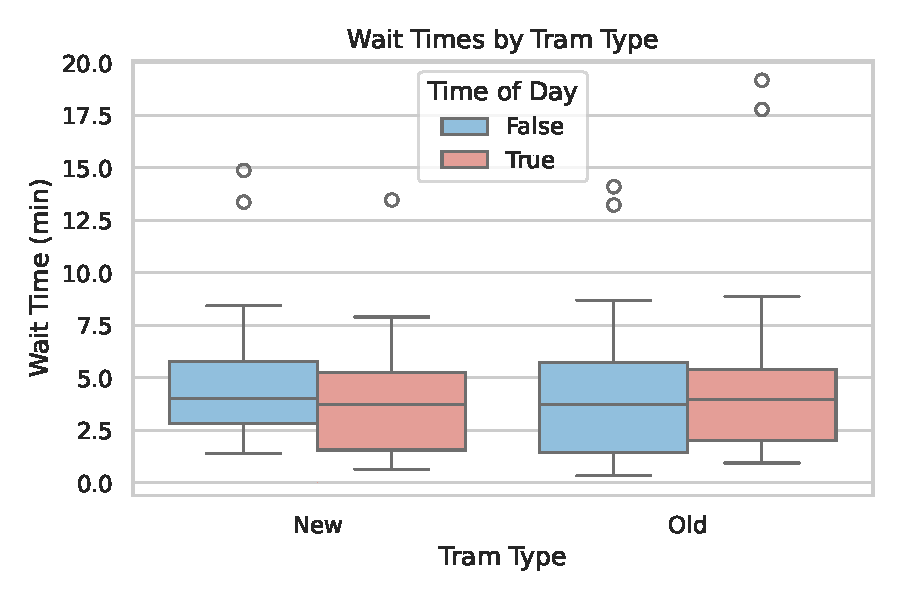
\includegraphics[width=\textwidth]{Plot_WaitTimesByTramType.pdf}
						\caption{Wait Times by Tram Type}
						\label{fig:wait_time_by_tram_type}
					\end{subfigure}
					\hfill
					\begin{subfigure}[b]{0.48\textwidth}
						\centering
						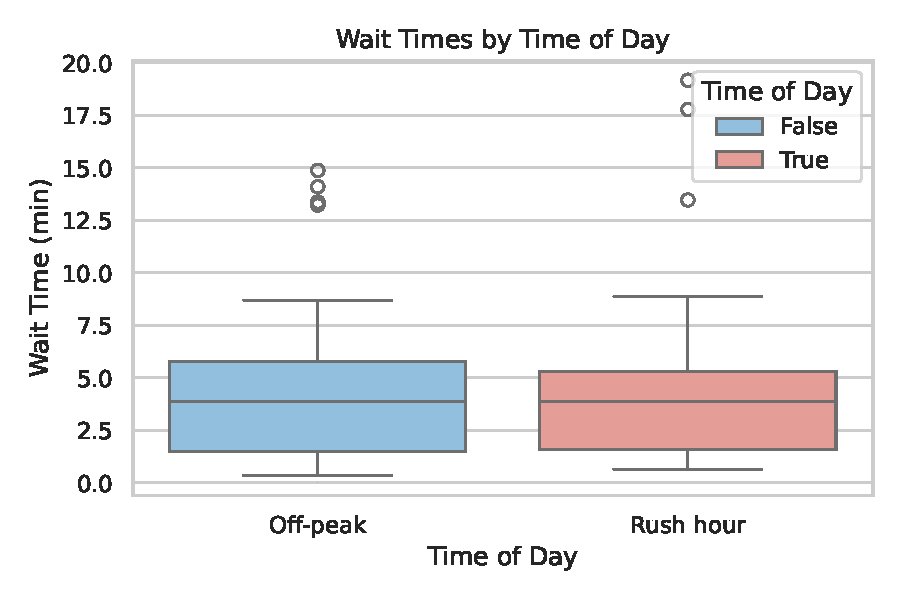
\includegraphics[width=\textwidth]{Plot_WaitTimesByTimeOfDay.pdf}
						\caption{Wait Times by Time of Day}
						\label{fig:wait_time_by_time_of_day}
					\end{subfigure}
						
					\caption{Boxplot of Tram Wait Times}
					\label{fig:wait_time_boxplots}
				\end{figure}

				\noindent The boxplots in Figure~\ref{fig:wait_time_boxplots} show that the wait times during
				rush hours are generally \textbf{shorter} than during non-rush hours! //

				\noindent However if we take a look at Figure~\ref{fig:wait_time_by_time_of_day} we will see that 
				non rush hour, or Off-peak, wait times generally have more \textbf{outliers} than rush hour wait times, but
				the rush hour wait times have \textbf{bigger outliers} than the non rush hour wait times. \\

				\noindent This means that the rush hour wait times are more \textbf{consistent} 
				than the non rush hour wait times, and this can also be seen by a somewhat smaller interquartile range (IQR) 
				for the rush hour wait times. \\

				\noindent If we also take a look at Figure~\ref{fig:wait_time_by_tram_type}, 
				we can see that the wait times for the new trams are generally 
				\textbf{shorter} than the wait times for the old trams. Also when it came to outliers, 
				the new trams and the old trams had a similar number of outliers, 
				but the new trams had \textbf{smaller outliers} than the old trams, especially during rush hours. \\

		\newpage
		\subsection{Tram Proportion}
				\noindent Another things we focused on was the proportion of old vs. new trams during rush hours and non-rush hours. \\

				\noindent As mentioned before in the introduction, the old trams are generally not accessible to people in wheelchairs,
				so it is important to see how many of the new trams are running during rush hours and non-rush hours. \\

				\begin{figure}[h!]
					\centering
					\begin{subfigure}[b]{0.48\textwidth}
						\centering
						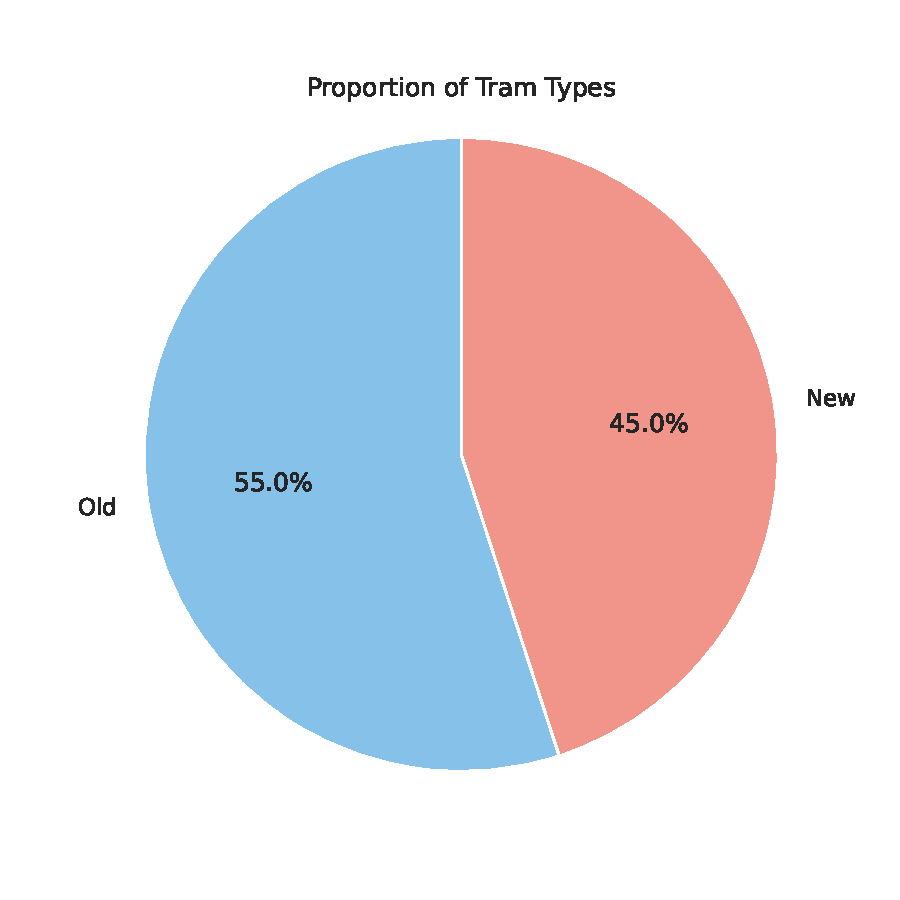
\includegraphics[width=\textwidth]{Plot_TramProportions.pdf}
						\caption{Proportion of Trams}
						\label{fig:proportion_of_trams_by_type}
					\end{subfigure}	
					\hfill
					\begin{subfigure}[b]{0.48\textwidth}
						\centering
						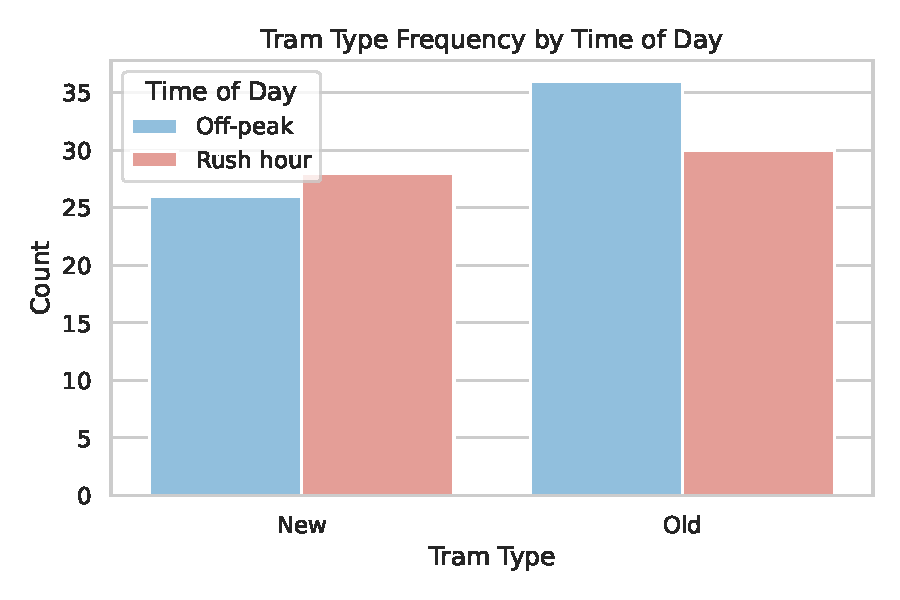
\includegraphics[width=\textwidth]{Plot_TramFrequencyByTimeOfDay.pdf}
						\caption{Proportion of Trams by Time of Day}
						\label{fig:proportion_of_trams_by_time_of_day}
					\end{subfigure}
				\end{figure}

				\noindent As can be seen in Figure~\ref{fig:proportion_of_trams_by_type} there does seem to be a slight difference in 
				the proportion of old vs. new trams during rush hours and non-rush hours, the question of if this is enough 
				to be statistically significant is answered in the next section. \\

				\noindent However if we take a look at Figure~\ref{fig:proportion_of_trams_by_time_of_day}, we can see that during
				non rush hours the proportion of old trams is significantly higher than then the proportion of new trams, which does
				cause a problem for people in wheelchairs, since the old trams are not accessible to them, hence causing them to 
				have to spend a longer time waiting. \\

		\newpage
		\subsection{Power Curve}
				\noindent Whilst the power curve doesn't give us any new information to work with, 
				however it does give us a good idea of how likely we are to reject the null of wait time being different during
				rush and non rush hours hypothesis correctly. \\

				\noindent Specifically our power curve in Figure~\ref{fig:power_curve} 
				will tell us to what extent the effect needs to be in order for us to be able to reject the null hypothesis with
				$80\%$ confidence. \\

				\begin{figure}[h!]
					\centering
					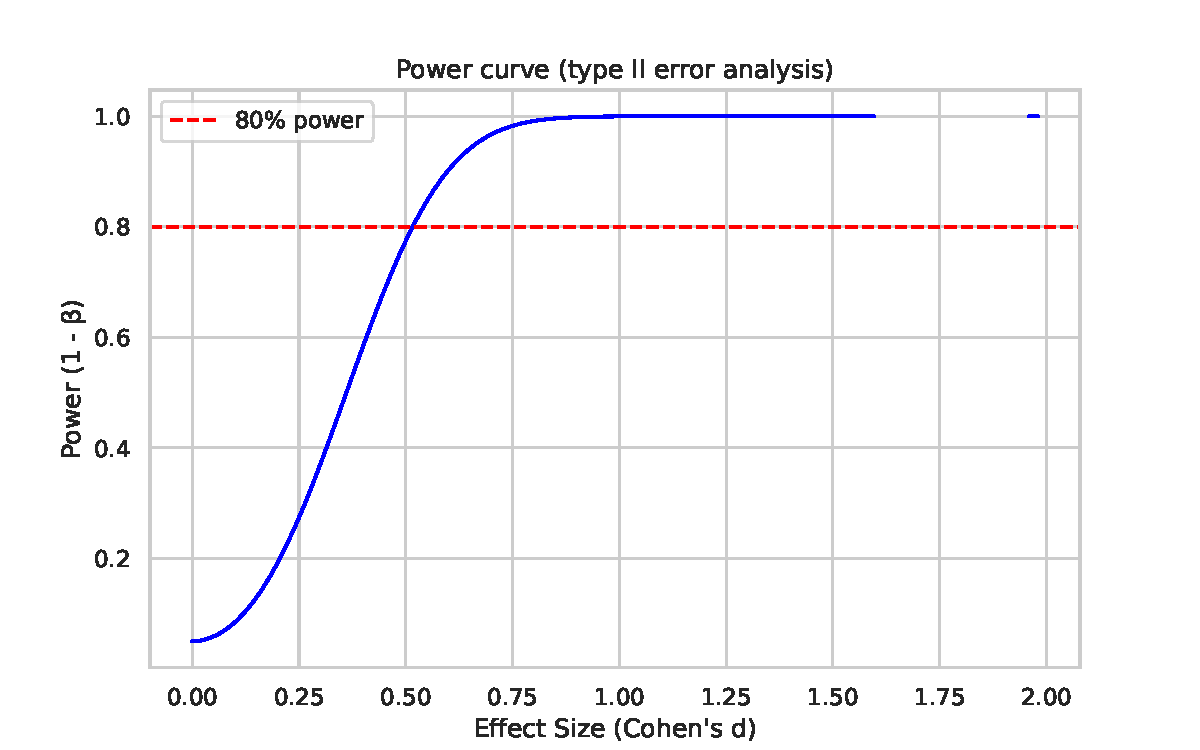
\includegraphics[width=0.9\textwidth]{Plot_PowerCurve.pdf}
					\caption{Power Curve for Tram Wait Time Analysis}
					\label{fig:power_curve}	
				\end{figure}

				\noindent As we can see the Cohen's $d$ value needs to be around $0.5$ in order for us to be able to reject the null 
				hypothesis with $80\%$ confidence. \\

				\noindent For more information on the power curve and how it was calculated, please refer to Appendix \ref{sec:power_analysis}.


	\section{Statistical Analysis and Hypothesis Testing}
		This Section will cover the statistical analysis and hypothesis testing we performed on the data collected. 
		The tests were performed using Python, and the code can be found in Appendix~\ref{sec:hypothesis_test_code}. \\

		\subsection{Proportion of Old vs. New Trams}
			\noindent To test the hypothesis regarding the proportion of old vs. new trams during 
			rush and non-rush hours, we used a \textbf{one-sample proportion z-test}. \\

			\noindent As mentioned in Section~\ref{sec:proportion_hypothesis}, our null hypothesis is that the proportion of old trams 
			during rush hours is equal to the proportion of old trams during non-rush hours. \\

			\noindent The reason we did not use a two-sample proportion z-test is because these two proportions are 
			\textit{not independent} of each other. Knowing the proportion of old trams automatically 
			determines the proportion of new trams, and vice versa, meaning the degrees of freedom is effectively one. \\
			\newpage

			\noindent Let us denote:
			\begin{itemize}
					\item \( P_{\text{old}} \) = proportion of old trams
					\item \( P_{\text{new}} \) = proportion of new trams
			\end{itemize}

			Since a tram is either old or new:
			\[
			P_{\text{old}} = 1 - P_{\text{new}}
			\]

			\noindent The null hypothesis \( H_0 \) is that the proportion of old trams is the same in both conditions:
			\[
			P_{\text{old}} = P_{\text{new}}
			\]

			\noindent Substituting using \( P_{\text{old}} = 1 - P_{\text{new}} \), we get:
			\[
			1 - P_{\text{new}} = 1 - P_{\text{new}}
			\Rightarrow P_{\text{new}} = P_{\text{new}}
			\]

			\noindent Therefore, for both the old and new tram proportions to be equal:
			\[
			P_{\text{new}} = \frac{1}{2} = 0.5 = 50\%
			\]

			\noindent Thus, testing whether the proportion is different from 50\% using a 
			one-sample proportion z-test is both valid and sufficient. \\ 

			\noindent The new hypothesis can be stated as: 
			\begin{align*}
				H_0: P_{\text{new}} &= 0.5 \\
				H_a: P_{\text{new}} &\neq 0.5
			\end{align*}

			\noindent We will also pick a significance level of \( \alpha = 0.05 \) for our test. \\

			After performing the one-sample proportion z-test these are the values we got:
			\begin{itemize}
				\item \textbf{Test Statistic:} \( z = -1.095 \)
				\item \textbf{p-value:} \( p = 0.273 \)
			\end{itemize}

			\noindent Since the p-value \( 0.273 \) is greater than our significance level \( \alpha = 0.05 \), 
			we \textbf{fail} to reject the null hypothesis.
		
		\subsection{Average Tram Wait Time (Overall)}
			\noindent To test the hypothesis regarding the average tram wait time, we used a \textbf{one-sample t-test}. \\

			\noindent As mentioned in Section~\ref{sec:wait_time_hypothesis}, our null hypothesis is that the average tram wait time is 4 minutes. \\

			\noindent The null and alternative hypotheses can be stated as:
			\begin{align*}
				H_0: \mu &= 4 \\
				H_a: \mu &\neq 4
			\end{align*}

			\noindent We will also pick a significance level of \( \alpha = 0.05 \) for our test. \\

			After performing the one-sample t-test these are the values we got:
			\begin{itemize}
				\item \textbf{Sample Mean:} \( \bar{x} = 4.421 \)
				\item \textbf{T-Statistic:} \( T = 1.358 \)
				\item \textbf{p-value:} \( p = 0.177 \)
			\end{itemize}

			\noindent We fail to reject the null hypothesis $H_0$ since the p-value \( 0.177 \) is greater than our 
			significance level \( \alpha = 0.05 \). \\

		\subsection{Average Wait Time: Rush vs. Non-Rush Hours}
			\noindent To test the hypothesis regarding the average wait time during rush hours vs. non-rush hours, 
			we used a \textbf{two-sample t-test}. \\

			\noindent As mentioned in Section~\ref{sec:wait_time_rush_non_rush_hypothesis}, 
			our null hypothesis is that the average wait time is the same during rush and non-rush hours. \\

			\noindent The null and alternative hypotheses can be stated as:
			\begin{align*}
				H_0: \mu_{\text{rush}} &= \mu_{\text{non-rush}} \\
				H_a: \mu_{\text{rush}} &\neq \mu_{\text{non-rush}}
			\end{align*}

			\noindent We will also pick a significance level of \( \alpha = 0.05 \) for our test. \\

			After performing the two-sample t-test these are the values we got:
			\begin{itemize}
				\item \textbf{Rush Hour Mean:} \( \bar{x}_{\text{rush}} = 4.406 \)
				\item \textbf{Non-Rush Hour Mean:} \( \bar{x}_{\text{non-rush}} = 4.434 \)
				\item \textbf{T-Statistic:} \( T = -0.045 \)
				\item \textbf{p-value:} \( p = 0.964 \)
			\end{itemize}

			\vspace{1mm}
			\noindent Since the p-value \( 0.964 \) is greater than our significance level \( \alpha = 0.05 \), 
			we \textbf{fail} to reject the null hypothesis $H_0$ and conclude that there is no significant difference in average
			wait times between rush and non-rush hours.

		\subsection{Tram Type Distribution by Time of Day}
			\noindent To test the hypothesis regarding the distribution of tram types by time of day, 
			we used a \textbf{Chi-Squared Test for Independence}. \\

			\noindent As mentioned in Section~\ref{sec:tram_type_distribution_hypothesis}, 
			our null hypothesis is that the time of day does not significantly affect the distribution of tram types. \\

			\noindent The null and alternative hypotheses can be stated as:
			\begin{align*}
				H_0: \text{Time of day} &\text{ does not affect tram type distribution} \\
				H_a: \text{Time of day} &\text{ affects tram type distribution}
			\end{align*}

			\noindent We will also pick a significance level of \( \alpha = 0.05 \) for our test. \\

			After performing the Chi-Squared Test for Independence these are the values we got:
			\begin{itemize}
				\item \textbf{Chi-Squared Statistic:} \( \chi^2 = 0.264 \)
				\item \textbf{p-value:} \( p = 0.607 \)
				\item \textbf{Degrees of Freedom:} \( df = 1 \)
			\end{itemize}

			\vspace{1mm}
			\noindent Since the p-value \( 0.607 \) is greater than our significance level \( \alpha = 0.05 \), 
			we \textbf{fail} to reject the null hypothesis $H_0$ and conclude that the time of day does not 
			significantly affect the distribution of tram types. \\

	\newpage
	\begin{appendices}
		\section{CSV Dataset Contents}
		\label{sec:rawdata}
		\input{Data/StatisticalAnalysisOfTrams.tex}

		\newpage
		\section{Power Analysis Code and Explanation}
		\label{sec:power_analysis}

		\subsection*{Python Code Used for Power Curve}
			\lstinputlisting[style=pythonstyle, caption={Proportion Curve Python Code}, label={lst:power_curve}]{Code/PowerCurve.py}	

			\subsection*{Explanation of Power Calculation}

				The statistical power of a test is defined as:

				\[
				\text{Power} = 1 - \beta
				\]

				where:
				\begin{itemize}
						\item \( \beta \) is the probability of a Type II error (failing to reject the null hypothesis when it is false).
						\item \( \alpha \) is the significance level (probability of a Type I error).
						\item Power is the probability that the test correctly rejects the null hypothesis when a true difference exists.
				\end{itemize}

				The effect size used here is \textbf{Cohen's \( d \)}, calculated as:

				\[
				d = \frac{|\mu_1 - \mu_2|}{\sigma_{\text{pooled}}}
				\]

				with \( \mu_1 \) and \( \mu_2 \) representing the means of tram wait times during rush hour and non-rush hour respectively, and \( \sigma_{\text{pooled}} \) being the pooled standard deviation.

			\subsection*{Purpose of the Power Curve}

				This power curve allows us to visualize how sensitive our statistical test is to differences in tram wait times. It shows the probability of detecting a real difference (if it exists) based on various hypothetical effect sizes. A commonly accepted threshold for adequate power is 0.8, meaning there's an 80\% chance the test will detect a true effect.

				\bigskip
				The analysis helps ensure that our sample size is sufficient to make confident conclusions regarding tram service differences during rush hours.
		

		\newpage
		\section{Hypothesis Test Code}
		\label{sec:hypothesis_test_code}
		  \noindent In this Appendix, we provide the Python code used to perform the hypothesis tests for both the average tram wait time and the proportion of old vs. new trams. The code is structured to be clear and easy to follow, with comments explaining each step of the process.

			\subsection*{Proportion of Old vs. New Trams}
				\lstinputlisting[style=pythonstyle, caption={Proportion Test Code}, label={lst:power_curve}]{Code/ProportionTest.py}	

			\newpage
			\subsection*{Average Tram Wait Time (Overall)}
				\lstinputlisting[style=pythonstyle, caption={Average Wait Time Test Code}, label={lst:average_wait_time}]{Code/AverageWaitTimeOverallTest.py}

			\newpage
			\subsection*{Average Wait Time: Rush vs. Non-Rush Hours}
				\lstinputlisting[style=pythonstyle, caption={Rush vs Non-Rush Wait Time Test Code}, label={lst:rush_vs_non_rush}]{Code/AverageWaitTimeRushVsNonRush.py}

			\newpage
			\subsection*{Tram Type Distribution by Time of Day}
				\lstinputlisting[style=pythonstyle, caption={Tram Type Distribution Test Code}, label={lst:tram_type_distribution}]{Code/TramTypeDistributionTest.py}
	\end{appendices}

\end{document}
